\subsection{Exodus, Volcano, Cascades}

Das Volcano Projekt mit seinem Vorgänger \ac{EXODUS} und dem Nachfolger Cascades bildet die Grundlage für den Microsoft SQL Server und dessen Anfrageoptimierer. Bei der Implementierung des Volcano Optimierers ist insbesondere die Implementierung des Query Optimierers von Interesse und wird daher ausführlich behandelt.

\subsubsection{Exodus}


Bereits in den 1970er Jahren begann Graefe mit der Implementierung eines DBMS Frameworks unter dem Titel EXODUS \cite{carey1990exodus} . Das Projekt, das die Grundlage für Volcano legen sollte, hatte sich zum Ziel gesetzt, einen erweiterbaren, applikationsspezifischen und hochperformanten Baukasten zusammenzustellen, mit dessen Hilfe neue Datenbanksysteme generiert werden konnten. 

Im Gegensatz zu konventionellen DBMS wie System R oder Starburst handelt es sich bei EXODUS nicht um ein funktionsfähiges und sofort einsatzfähiges DBMS, sondern um einen Baukasten, auf dessen Basis ein neues System durch einen \ac{DBI} erstellt werden kann. Im Gegensatz zu anwendungsübergreifend designten DBMS wie Postgres bietet EXODUS den Vorteil, dass eine Datenbank speziell an die Bedürfnisse eines Anwendungsfalles angepasst ist und so die Anforderungen einer Anwendung passgenau erfüllt. Um dennoch das Ziel der Performance nicht aus den Augen zu verlieren, werden viele Komponenten nicht immer wieder auf einer grünen Wiese entwickelt, sondern auf dem Fundament des EXODUS Baukastens aufgebaut.

\begin{figure}[ht]
  \centering
  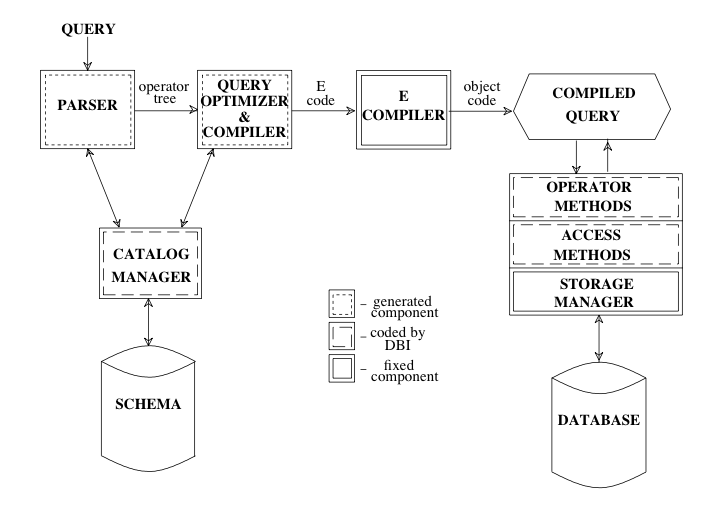
\includegraphics[width=\textwidth]{02_Related_Work/ExodusDatabaseSystemStructure.png}
  \caption{Exodus Database System Structure}
  \label{ExodusDatabaseStructure}
\end{figure}\todo{Eigene Grafik bauen}

Der Baukasten von EXODUS besteht aus drei Arten von Bausteinen: Bausteine die fix vorgegeben und nicht verändert werden sollen, Bausteinen, die speziell entwickelt werden müssen und Teilen, die generiert werden. Der Werkzeugkasten umfasst dabei nicht nur die Bausteine, sondern auch die Werkzeuge zur Bearbeitung und Generierung. Zu den Werkzeugen gehören ein Tool zur Erstellung eines Front-Ends für die Anfragesprache, ein Query Optimizer Generator und die Programmiersprache E (zusammen mit einem passenden Compiler). Mit Hilfe des Tools zur Erstellung eines Front-Ends für Anfragesprachen kann die Parser Komponente generiert werden. Der Query Optimizer wird als Resultat des Query Optimizer Generators erzeugt. (vgl. \ref{ExodusDatabaseStructure})

Neben den generierten Komponenten gibt es den E Compiler, der E Code in Objekt-Code übersetzt. Er kommt zum Einsatz, um die durch den Query Optimizer optimierte Anfrage in eine kompilierte Anfrage umzusetzen. Diese Komponente ist ähnlich wie der Storage Manager, der für die Verwaltung von Daten in der Datenbank genutzt wird, unveränderlich. 

Zwischen der kompilierten Anfrage und dem Storage Manager kommen zwei Komponenten zum Einsatz, die von einem DBI geschrieben werden müssen: Die Operator Methoden und Access Methoden. Diese beiden Komponenten dienen dazu, die Anfrage in Code zu übersetzen, der durch den  Storage Manager ausgeführt wird.

Bei der Implementierung eines Optimierers kommen grundsätzlich zwei mögliche Ansätze in Frage: (1) interpretierte und (2) kompilierte Programmiersprachen. Bei EXODUS wurde zuerst die Implementierung mittels sog.\"AI\" Sprachen versucht. In einem Prototypen wurde mit Hilfe von Prolog ein Optimierer entwickelt. Für Prolog hat man sich entschieden, da diese Sprache Pattern Matching und eine Search Engine bereitstellt. (Auch unification konnte zum Einsatz gebracht werden, um elegant Query Trees zu erstellen.) Der Hauptvorteil eines interpretierten Ansatzes war aus Sicht von EXODUS die Möglichkeit neue Regeln zur Laufzeit des Programms hinzuzufügen. Trotz dieser Vorteile wurde der Ansatz als zu langsam verworfen. Auch der Vorteil Regeln während der Laufzeit hinzuzufügen, wird in der Literatur \todo{QUELLE} als wenig nützlich bewertet. Statt dieses Ansatzes wurde in der Folge auf die Erstellung eines Generators, der in C geschrieben wurde, gesetzt. Der Generator erstellt basierend auf Regeln einen Optimierer in C, der wiederum kompiliert werden kann. Zwar war die Entwicklung des C Generators aufwändiger als die Implementierung in Prolog, jedoch konnte auf applikationsspezifische Notwendigkeiten, wie die Implementierung von speziellen Suchverfahren, punktgenau eingegangen werden.


Die Generierung des Optimierters geschieht auf Basis eines Description-Files. Dieses File setzt sich aus drei Komponenten zusammen: Operatoren, Methoden und Regeln.


Die Operatoren bezeichnen die logische Algebra. Die Methoden werden in der physischen Algebra verwendet. Ebenfalls sind Transformationen Teil des Description-Files. Es wird zwischen zwei Arten an Regeln unterschieden: Transformationsregeln und Implementierungsregeln. Implementierungsregeln kommen bei der Übersetzung von logischer in physische Algebra zum Einsatz. Transformationsregeln sind für die Erzeugung von alternativen Plänen verantwortlich.

Allen Regeln ist gemein, dass sie wie bereits beschrieben aus zwei Teilen bestehen. Einer Methode, die in C geschrieben ist, die prüft, ob eine Regel angewendet werden kann und einer Transformation, die auf einer algebraischen Äquivalenz basiert. Der linke Teil der Äquivalenz stellt dabei die Eingabe der Transformation dar, der rechte Teil der Äquivalenz den Output der durch Transformation entstanden ist. Neben dieser deklarativen Implementierung von Regeln ist es auch möglich komplexere Regeln mit Hilfe von C Routinen zu entwickeln.

Diese Regeln werden gemeinsam mit Hilfe des Optimizer Generators in C Code umgewandelt, der dann wie jeder andere Query-Optimizer verwendet werden kann. 

Bei der Anwendung der Regeln wird zuerst geprüft, welche Regeln anwendbar sind. Diese Regeln werden in der Liste OPEN abgelegt. Durch einen Auswahlmechanismus wird festgelegt, welche Regel zum Einsatz kommt. Nachdem eine Regel angewendet wurde, wird sie aus der OPEN Liste entfernt. Regelanwendungen, die durch diese Transformation möglich wurden, werden der OPEN Liste hinzugefügt. Der Auswahlmechanismus sieht vor, dass die potenziell gebildeteten Pläne auf Grund ihrer Kosten bewertet werden und die Regel ausgeführt wird, die zum günstigsten Plan führt. Die Suchstrategie wird als Hill climbing bezeichnet.

Einer der Nachteile dieses Ansatzes ist es, dass Pläne nicht bzgl. ihrer Güte auf einem globalen Level bewertet werden können. Es ist nicht möglich festzustellen, ob es sich um den absolut günstigsten Plan handelt, da weitere Transformationen noch angewendet werden können. Auch Kostenreduktionen, die erst durch die Kombination mehrerer Regeln entstehen, werden nicht berücksichtigt. Auch Graefe selbst sieht einige weitere Nachteile \cite{graefe1993volcano}:

\begin{itemize}
\item nicht-triviale Kostenmodelle
\item keine Eigenschaften
\item keine Heuristiken
\item keine Transformation von Subscripten von algebraischen Operatoren nach algebraische Operatoren
\end{itemize}


\subsubsection{Volcano Optimizer}

Volcano ist der verbesserte Nachfolger von EXODUS. Zuerst war Volcano nur ein erweiterbares, paralleles System zur Anfragenausführung. Später wurde ein neuer Anfrageoptimierer-Generator hinzugefügt. Im Gegensatz zu der bisher verwendeteten Programmiersprache E in der der Optimierer erzeugt wurde, setzt das Projekt auf C Code. 


Bei der Generierung eines Plans auf Grund einer Anfrage kommt bei Volcano ein Optimierer zur Anwendung, der speziell für den Anwendungsfall generiert wurde. Der Optimierer ist das Resultat einer Model Spezifikation, die von einem \ac{DBI} erstellt und durch einen Optimierer Generator in Source Code umgewandelt wird. Dieser Code wird mit Hilfe eines Compilers in das Endprodukt, den Optimierer, umgewandelt.


Der Volcano Optimizer wurde von Grund auf neu entwickelt und begegnet den von Graefe identifizierten Nachteilen des EXODUS Optimizer Generators. Ebenfalls wird die Arbeit mit der Sprache E eingestellt und vollumfänglich auf C gesetzt. Die Verbesserungen werden in fünf fundamentalen Designentscheidungen\cite{graefe1993volcano} sichbar, die eine effiziente Suche des Optimierers erlauben:


\begin{enumerate}

\item Die erste Grundlage des Volcano Optimierers ist die Anwendung von algebraischen Techniken wie algebraische Operatoren und Äquivalenzklassen. Volcano unterscheidet dabei zwischen logischer und physischer Algebra. Die Umwandlung von logischer Algebra (der Anfrage) in die physische Algebra (einem Query Evaluation Plans) geschieht durch die Transformation der logischen Algebra mit Hilfe von kostenbasierten Mappings von logischen Algorithmen. \todo{Unklar}


\item Das zweite Prinzip sieht vor, dass die Information über algebraische Gesetze, die zur Transformation von Algebraischen Ausdrücken genutzt werden als Regeln und Pattern modular erfasst sind. Durch dieses Prinzip sind die einzelnen Regeln klar und transparent von einander getrennt und können zu Regelsets zusammengestellt werden. Einige dieser Regelsets werden im folgenden Kapitel behandelt.


\item Das dritte Prinzip betrifft die Eingabe des Optimierers. Im Gegensatz zu anderen Optimierern (namentlich Starbust) setzt der Volcano Optimizer auf algebraische Äquivalenzen als Eingabe Parameter. Andere Systeme nutzen hier mehrere Stufen an Umwandlung, um zwischen Query und Optimizer Eingabe zu vermitteln. 

\item Kompilierung über Interpretierung von Regeln ist das vierte Prinzip, das zur Anwendung kommt. Da es sich bei der Generierung von äquivalenten Plänen um ein CPU intensives Geschäft handelt, wurde entschieden, dass die Regeln zur Transformation der Pläne kompiliert und nicht interpretiert werden. Zwar verliert der Optimierer daduch die Möglichkeit ad hoc neue Regeln in den Optimierer aufzunehmen. Jedoch wird diese Möglichkeit in der Praxis nicht benötigt. 

\item Das letzte Prinzip ist, dass der Volcano Optimierer auf dynamisches Programmieren bei der Generierung von Programmen setzt. \todo{Unklar}
\end{enumerate}


Wie bereits zuvor wird der Ausdruck in einen Operatorbaum umgewandelt. Transformationsregeln und Implementierungsregeln kommen bei der Optimierung zum Einsatz. Eine Trennung zwischen Optimierung auf logischer und auf physischer Ebene findet nicht statt. Es wird zuerst ein logischer Ast erzeugt, für den dann unterschiedliche physische Pläne generiert werden. Diese Pläne werden auf der Basis ihrer Kosten verglichen, nur der günstigste Plan bleibt bestehen und wird gespeichert. Ist bereits ein Plan vorhanden, so wird nur der günstigste Plan im Speicher behalten. Bei der Generierung kommt zudem eine Memo-Struktur zum Einsatz. In einer Hashtabelle wird geprüft ob eine Transformation bereits bekannt ist. Wenn das der Fall ist, wird diese Transformation verwendet und somit doppelter Berechnungsaufwand gespart und die bekannte Transformation stattdessen referenziert.

Regeln und insbesondere Transformationsregeln, die bei der Transformation im Bereich JOIN-Reihenfolgeänderung verwendet werden, werden in \ref{sec:pellenkoftRulesets} beschrieben.

